\begin{figure}[t]
\centering
% Vector drawing generated by tools/figures/extraction.py; rerun it after changing the figure.
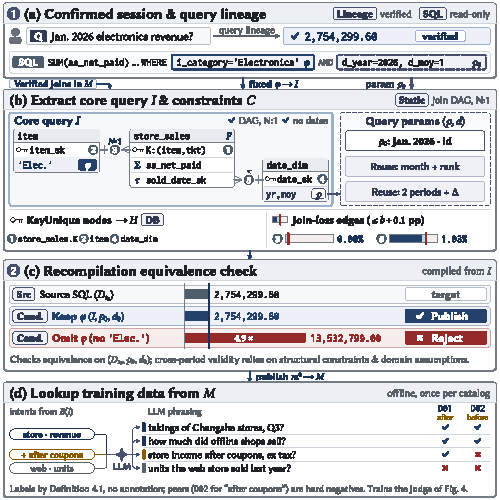
\includegraphics[width=0.92\columnwidth]{figures/extraction}%
\caption{\bt{Graph-based agent knowledge extraction (steps 1--2): grounded in the dependency graph $\mathcal{G}$, the candidate retaining scope filter $\varphi$ passes recompilation equivalence on $D_{s_0}$; the incomplete draft is rejected.}{基于图的智能体知识提取（步骤 1--2）：在依赖图 $\mathcal{G}$ 中对齐并保留范围过滤 $\varphi$ 的候选于源快照 $D_{s_0}$ 通过重编译等价性验证，遗漏该过滤的草稿被拒绝。}}
\label{fig:extraction}
\Description{Three panels read from top to bottom. (a) Agent 1's confirmed January 2026 electronics-revenue session returns 2,754,299.60, together with its query lineage, verified as read-only source SQL without reading base-table rows. (b) Aligned with verified join paths in M, the extracted core query I fixes store_sales at item-ticket grain, SUM(ss_net_paid), sale-date attribution, many-to-one acyclic joins to item and date_dim, and the mandatory Electronics category filter phi. Query parameters are p0 equal to January 2026 and d0 equal to identity; later requests can bind a month and ranking, or two periods and a difference. Static structural checks validate the join DAG. PostgreSQL checks key uniqueness and derives constraint nodes C into H: 1 fact-grain uniqueness, 2 item-key uniqueness, 4 date-key uniqueness, plus join-loss edges 3 item-join loss and 5 date-join loss, numbered consistently with Figure 5. (c) Recompilation equivalence checks source SQL against recompiling I with p0 and d0 alone. Retaining phi yields 2,754,299.60 and permits publication; omitting phi yields 13,532,799.00 and is rejected. Equivalence is checked on the learning snapshot and binding, while cross-period validity relies on structural constraints and domain assumptions.}
\end{figure}
